% IN6227 Assignment 1, Variant 2 -- Overleaf copy of the SKILL-generated report.
% Compile with pdfLaTeX. This single file needs no external figures or .bib file.
% Every number below is copied from the verified RUN-008 artifacts; the
% machine-readable sources are report/report_data.json, test_metrics.json,
% cv_results.csv and verification.json. If the SKILL is rerun, regenerate this
% file instead of editing numbers by hand.
% Keep the separate Reflection outside the two-page main report.

\documentclass[10pt,a4paper,twocolumn]{article}

\usepackage[left=0.72in,right=0.72in,top=0.95in,bottom=0.95in]{geometry}
\setlength{\columnsep}{0.22in}
\usepackage[T1]{fontenc}
\usepackage{newtxtext,newtxmath}
\usepackage{microtype}
\usepackage{booktabs,tabularx,array,colortbl}
\usepackage{balance}
\usepackage[font=small,labelfont=bf,hypcap=false]{caption}
\usepackage{titlesec}
\usepackage{fancyhdr}
\usepackage{xurl}
\usepackage{pgfplots}
\pgfplotsset{compat=1.18}
\usepackage[colorlinks=true,urlcolor=blue!55!black,linkcolor=black]{hyperref}

\definecolor{ink}{RGB}{31,42,55}
\definecolor{muted}{RGB}{92,103,115}
\definecolor{barA}{RGB}{54,86,131}
\definecolor{barB}{RGB}{191,120,58}

% Table columns: a wider label column with evenly divided numeric columns,
% so the values sit under their headings instead of drifting to the margin.
\newcolumntype{L}{>{\raggedright\arraybackslash\hsize=1.5\hsize}X}
\newcolumntype{C}{>{\centering\arraybackslash\hsize=0.875\hsize}X}
\newcolumntype{M}{>{\raggedright\arraybackslash\hsize=1.6\hsize}X}
\newcolumntype{D}{>{\centering\arraybackslash\hsize=0.68\hsize}X}

\titleformat{\section}{\normalfont\fontsize{10}{12}\selectfont\bfseries\color{ink}}{}{0pt}{}
\titlespacing*{\section}{0pt}{5pt}{1.5pt}
\setlength{\parindent}{1em}
\setlength{\parskip}{0.5pt}
\setlength{\tabcolsep}{3.5pt}
\renewcommand{\arraystretch}{1.12}
\raggedbottom

\pagestyle{fancy}
\fancyhf{}
\fancyhead[L]{\fontsize{8}{10}\selectfont\color{muted}IN6227 Data Mining / Assignment 1 / Variant 2}
\fancyfoot[L]{\fontsize{8}{10}\selectfont\color{muted}HU YINGXIN}
\fancyfoot[R]{\fontsize{8}{10}\selectfont\color{muted}\thepage}
\renewcommand{\headrulewidth}{0pt}
\renewcommand{\footrulewidth}{0pt}
\setlength{\headheight}{11pt}

\begin{document}
\twocolumn[{%
  \begin{center}
    {\fontsize{19}{22}\selectfont\bfseries\color{ink}Leakage-Aware Tabular Classification\par}
    \vspace{5pt}
    {\fontsize{10}{12}\selectfont HU YINGXIN \quad G2608370F\par}
    {\fontsize{10}{12}\selectfont IN6227-Assignment-1 \quad Variant-2\par}
    \vspace{2pt}
    {\fontsize{8.5}{10}\selectfont\color{muted}
      LLM: \texttt{gpt-5.6-sol} (GPT-5.6 Sol) \quad
      Reasoning effort: medium \quad Interface: Codex Desktop\par}
    {\fontsize{8.5}{10}\selectfont\color{muted}
      Skill Markdown: \href{https://github.com/js25040304-ship-it/IN6227-assignment-1}{GitHub repository}\par}
  \end{center}
  \vspace{3pt}
  \hrule height 0.5pt
  \vspace{8pt}
}]

\balance

\section*{DATA AND CLEANING}
The supplied archive contained one binary target, \texttt{label}
(\texttt{yes}/\texttt{no}), and 15 predictors: seven numeric and eight
categorical. Rows without a label cannot supervise training, so they were
excluded before modelling: three from the development split and one from the
test split. That left 31,109 development rows and 13,333 test rows.

\noindent
\begin{minipage}{\columnwidth}
\centering
\captionof{table}{Verified data profile for the two supplied splits.}
\label{tab:profile}
\vspace{2pt}
{\normalsize
\begin{tabularx}{\columnwidth}{@{}MDDDDD@{}}
\toprule
\rowcolor{barA!10}
Split & Usable & Miss. & Miss. & Dup. & IQR \\
 & rows & label & pred. & rows & flags \\
\midrule
Development & 31,109 & 3 & 50 & 0 & 10,908 \\
Test & 13,333 & 1 & 21 & 0 & 4,762 \\
\bottomrule
\end{tabularx}}
\end{minipage}
\par\vspace{5pt}

The positive class was 24.0\% of development rows and 23.8\% of test rows. A
majority-to-minority ratio of 3.17:1 means a classifier can reach 76\%
accuracy by always answering \texttt{no}, so accuracy alone was never used to
judge a model. Missing predictors affected roughly 0.16\% of rows in each
split, and neither split contained duplicate rows; no test row shared its
complete predictor vector with a development row, so there was no evidence of
train/test row overlap.

Distribution checks flagged 10,908 IQR-extreme \emph{values} in development,
but the flags are concentrated rather than diffuse: \texttt{activity\_duration}
(5,350) and \texttt{load\_ratio} (2,527) supply 72\% of them, which points to
skewed distributions in two variables rather than corrupted records. Test
profiling flagged 4,762 values, a similar density (35.7 vs.\ 35.1 flags per
100 rows), so the two splits behave comparably. No row was deleted on
outlier evidence: with a 3.17:1 imbalance, blanket deletion removes
minority-class examples the model needs most.

Three numeric predictors were strongly correlated: \texttt{performance\_score}
with \texttt{stability\_index} (0.891), and both with \texttt{composite\_rank}
(0.880 and 0.830). Correlated inputs were retained for the tree model and read
cautiously for logistic regression, where coefficients are not treated as
independent effects.

\section*{PREPROCESSING AND FEATURES}
Numeric predictors were median-imputed and categorical predictors
most-frequent-imputed, in both cases fitted inside the training part of each
fold so that no validation row influenced its own imputation. Categorical
levels were one-hot encoded with unseen-category handling, a minimum level
frequency of two and a cap of 100 levels per field; the test split contained
no unseen categories. Only logistic regression used numeric scaling. Every
learned transformation stayed inside the five shuffled stratified folds
(seed 42).

The aggregate-like predictor \texttt{composite\_rank} was correlated with the
numeric predictors it could plausibly be derived from, and the dataset
documentation did not establish that it exists at prediction time. A
development-only sensitivity check changed macro-F1 by $+0.0002$ for logistic
regression and $-0.0011$ for random forest when the feature was removed. Both
shifts are smaller than the corresponding fold standard deviations (0.0079
and 0.0039), so the feature carried no measurable benefit while carrying
unresolved leakage risk. It was dropped before final evaluation, and the
final pipelines use the remaining 14 predictors. The check used development
folds only and cannot certify that the other 14 fields are available at
deployment.

\section*{TRAINING AND SELECTION}
Three configurations were compared on identical fixed folds: a
most-frequent dummy baseline, regularised logistic regression as an
interpretable linear reference, and a random forest as the nonlinear
challenger~[1]. The forest was the sensible challenger because eight of the
fifteen predictors are categorical and interactions between them are
plausible after bounded one-hot encoding.

The search space was fixed in advance. Logistic regression crossed
$C\in\{0.1,1.0\}$ with balanced versus unweighted class
treatment, four settings. The random forest used four joint settings rather
than a full grid: the class-weight choice is coupled to the leaf size
(balanced subsample with minimum leaf size 3, or unweighted with minimum leaf
size 1), and each pair was crossed with depth 18 versus unlimited, at 160
trees and square-root feature sampling. Every candidate was fitted with and
without \texttt{composite\_rank}, giving 17 candidate configurations in total
(1 dummy, 8 logistic, 8 forest) and 85 fold fits. Search stopped once that
predefined grid had been evaluated once.

Macro-F1 was the primary selection metric because it weights the two classes
equally and therefore cannot be improved by ignoring the minority
class~[3]. Selection used the paired development-fold difference with a
predefined one-standard-error practical-tie rule. Final-test metrics did not
inform any feature, parameter, threshold or model choice.

\section*{RESULTS}
\noindent
\begin{minipage}{\columnwidth}
\centering
\captionof{table}{Development and held-out comparison (forest selected).}
\label{tab:models}
\vspace{2pt}
{\normalsize
\begin{tabularx}{\columnwidth}{@{}LCCCC@{}}
\toprule
\rowcolor{barA!10}
Model & CV M-F1 & Test M-F1 & Yes rec. & Yes prec. \\
\midrule
Dummy & 0.432 & 0.433 & 0.000 & -- \\
Logistic & 0.761 & 0.762 & 0.570 & 0.696 \\
Random forest & \textbf{0.770} & \textbf{0.769} & \textbf{0.772} & 0.584 \\
\bottomrule
\end{tabularx}}
\end{minipage}
\par\vspace{6pt}

\noindent
\begin{minipage}{\columnwidth}
\centering
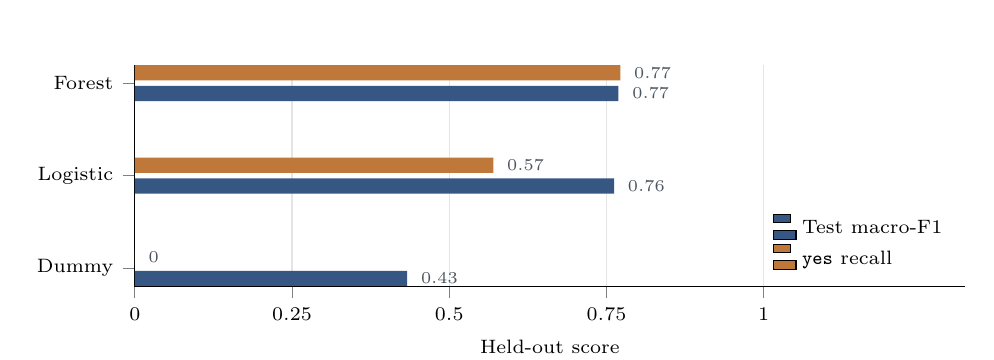
\begin{tikzpicture}[font=\fontsize{7.5}{9}\selectfont]
\begin{axis}[
  width=\columnwidth,
  height=4.4cm,
  xbar,
  bar width=5.5pt,
  xmin=0, xmax=1.32,
  xtick={0,0.25,0.5,0.75,1},
  xticklabel style={font=\fontsize{7}{8}\selectfont},
  xlabel={\fontsize{7}{8}\selectfont Held-out score},
  symbolic y coords={Dummy,Logistic,Forest},
  ytick=data,
  yticklabel style={font=\fontsize{7.5}{9}\selectfont},
  nodes near coords={\pgfmathprintnumber[fixed,precision=2]{\pgfplotspointmeta}},
  every node near coord/.append style={font=\fontsize{6}{7}\selectfont,color=ink!80,anchor=west,xshift=1.5pt},
  xmajorgrids=true,
  grid style={draw=black!10},
  axis lines*=left,
  tick align=outside,
  legend style={font=\fontsize{7}{8.5}\selectfont,draw=none,fill=none,at={(0.99,0.03)},anchor=south east},
  legend cell align=left,
]
\addplot[fill=barA,draw=none] coordinates {(0.433,Dummy) (0.762,Logistic) (0.769,Forest)};
\addplot[fill=barB,draw=none] coordinates {(0.000,Dummy) (0.570,Logistic) (0.772,Forest)};
\legend{Test macro-F1, \texttt{yes} recall}
\end{axis}
\end{tikzpicture}
\captionof{figure}{Held-out macro-F1 against positive-class recall.}
\label{fig:metrics}
\end{minipage}
\par\vspace{6pt}

\noindent
\begin{minipage}{\columnwidth}
\centering
\captionof{table}{Held-out confusion counts (\texttt{yes} positive).}
\label{tab:confusion}
\vspace{2pt}
{\normalsize
\begin{tabularx}{\columnwidth}{@{}LCCCC@{}}
\toprule
\rowcolor{barA!10}
Model & TN & FP & FN & TP \\
\midrule
Logistic & 9,378 & 787 & 1,363 & 1,805 \\
Forest & 8,425 & 1,740 & 723 & 2,445 \\
\bottomrule
\end{tabularx}}
\end{minipage}

The dummy baseline is a real floor, not a straw man: answering \texttt{no}
everywhere returns 0.762 accuracy but macro-F1 0.433 and balanced accuracy
0.500, and its average precision (0.238) is essentially the class prevalence.
Both substantive models clear it on the class-balanced measures (balanced
accuracy 0.800 and 0.746).

\section*{FINDINGS AND DISCUSSION}
The forest won on development evidence and reproduced that lead on the
held-out split: macro-F1 0.770 versus 0.761 across folds, and 0.769 versus
0.762 on test, with balanced accuracy 0.800. The gain is not free. The forest
recovered 77.2\% of positive cases against 57.0\% for logistic regression
(640 fewer false negatives) but raised 953 more false positives, giving lower
positive precision (0.584 versus 0.696) and lower accuracy (0.815 versus
0.839). Per class it is better on \texttt{yes} (F1 0.665 versus 0.627) and
worse on \texttt{no} (0.872 versus 0.897).

Ranking quality is a separate question from the decision rule. ROC-AUC was
0.889 for both models and average precision was 0.703 versus 0.702, so the two
models order the held-out rows almost identically; the visible difference
comes from where each untuned decision point falls, not from one model
separating the classes better. Reporting only accuracy, or only AUC, would
have hidden that distinction.

Across paired folds the forest-minus-logistic macro-F1 difference was
$+0.0093$ (SD 0.0111, SE 0.0050) and the forest won four of five folds. That
clears the practical-tie rule, but the rule is not a significance test: folds
share training data and a one-point gain is modest. Forest has the lower
observed error cost only if a false negative costs more than
$953/640\approx1.49$ times a false positive; this comparison is post hoc and
explains the choice rather than driving it.

No threshold tuning was attempted: the assignment supplies no error costs and
the held-out split has already been inspected, so a cost-driven threshold
chosen now would turn that evidence into another tuning resource. The
defensible next step is a fresh development-only plan with the deployment
costs written down first. Until then the forest is a reproducible research
choice under macro-F1, not an endorsed operational policy.

The analysis assumes independent rows and a stable train/test collection. No
dependency warning was raised, but that is not evidence of independence:
shared entities or a time order would need group- or time-aware validation.
The results also do not establish causal effects, fairness across unobserved
groups, probability calibration, or prediction-time availability for every
retained field, so generalization beyond this split remains conditional.

\section*{SKILL GENERALISATION}
The report is produced by a reusable SKILL. It takes a dataset path, profiles
the data, records typed quality warnings, selects preprocessing and two
substantive candidates from a fixed policy, evaluates them in fixed folds
against a dummy baseline, and writes a run directory of machine-readable
artefacts from which the report is rendered.

Generality was tested, not asserted. Eight synthetic cases ran end to end:
four modelling cases (numeric-only binary, mixed-type three-class, missing
values with an unseen category, imbalanced binary) each completed profiling,
comparison, verification and two-page report generation; two cases with an
ambiguous or absent target returned \texttt{needs\_input}; and two unsafe
cases refused rather than fabricating results.

\section*{VERIFICATION}
RUN-008 records dataset and Skill fingerprints, the seed, fold assignments,
candidate settings, saved predictions and package versions (Python 3.13.4,
pandas 2.2.3, NumPy 2.5.3, scikit-learn 1.9.1~[2]), together with ten
recorded decisions (DPROF-001--005, DMOD-001--005). An independent verifier
recomputed 54 checks from the saved predictions, covering all scalar metrics,
both confusion matrices, prediction-row alignment and score normalisation;
all passed. Two checks are explicit: the forest confusion counts sum to
13,333, and its positive recall is $2{,}445/(2{,}445+723)=0.772$. Reproducing
a run verifies the computation, not the provenance assumptions above.

\section*{REFERENCES}
{\footnotesize
\setlength{\parindent}{0pt}
\setlength{\parskip}{2pt}
\hangindent=1.4em
[1] Breiman, L. (2001). Random forests. \emph{Machine Learning}, 45(1), 5--32.
\href{https://doi.org/10.1023/A:1010933404324}{doi:10.1023/A:1010933404324}.\par
\hangindent=1.4em
[2] Pedregosa, F., et al. (2011). Scikit-learn: Machine learning in Python.
\emph{J.\ Mach.\ Learn.\ Res.}, 12, 2825--2830.\par
\hangindent=1.4em
[3] He, H., \& Garcia, E. A. (2009). Learning from imbalanced data.
\emph{IEEE Trans.\ Knowl.\ Data Eng.}, 21(9).
\href{https://doi.org/10.1109/TKDE.2008.239}{doi:10.1109/TKDE.2008.239}.\par
}

\end{document}
